\documentclass[10pt,twocolumn,letterpaper]{article}

% \usepackage{style/dicta}
% \def\dictaPaperID{xxxx} % *** Enter the DICTA Paper ID here
% \dictafinalcopy % *** Uncomment this line for the final submission

\usepackage{style/dlcc}
\def\dlccPaperID{0001} % *** Enter the DLCC Paper ID here
% \dlccfinalcopy % *** Uncomment this line for the final submission

\usepackage{times}
\usepackage{epsfig}
\usepackage{graphicx}
\usepackage{amsmath}
\usepackage{amssymb}
\usepackage{booktabs}
\usepackage{microtype}
\usepackage[pagebackref=true,breaklinks=true,letterpaper=true,colorlinks,bookmarks=false]{hyperref}

\def\httilde{\mbox{\tt\raisebox{-.5ex}{\symbol{126}}}}

% Pages are numbered in submission mode, and unnumbered in camera-ready
% \ifdictafinal\pagestyle{empty}\fi
\ifdlccfinal\pagestyle{empty}\fi

\begin{document}

%%%%%%%%% TITLE
\title{Data Augmentation Eliminates Double Descent:\\A Mechanistic Study on ResNet with CIFAR-10}

\author{Anonymous Authors\\
COMP5329 Deep Learning, University of Sydney\\
}

\maketitle

%%%%%%%%% ABSTRACT
\begin{abstract}
The double descent phenomenon---wherein test error rises near the interpolation threshold before falling again---challenges classical bias-variance intuitions about over-parameterization. While data augmentation is widely known to improve generalization, its mechanistic effect on the double descent curve has received little systematic study. We train ResNet and MLP models across seven parameter scales (11K--2.78M) with five augmentation strategies (None, Flip+Crop, Cutout, MixUp, Color Jitter) on CIFAR-10, repeated over three random seeds. We find that \textbf{ResNets without augmentation exhibit a clear double descent}, with test error peaking at $\sim$697K parameters (0.1144) before rising further to 0.1331 at 2.78M. All four augmentation strategies completely eliminate this peak, yielding monotonically decreasing error curves with test error as low as 0.0407 at 2.78M (MixUp). In contrast, \textbf{MLPs show no double descent} regardless of augmentation, suggesting this phenomenon is specific to convolutional architectures. A MixUp intensity ablation reveals negligible sensitivity to $\alpha \in [0.1, 1.0]$ (differences $<$0.0001), a negative result that constrains mechanistic accounts. Experiments on CIFAR-100 confirm that augmentation benefits scale with task difficulty, with Cutout reducing error by 36.7\% relative to no augmentation at 2.78M parameters.
\end{abstract}


%%%%%%%%% BODY TEXT
\section{Introduction}

A foundational principle of statistical learning holds that models with more parameters than training samples will overfit and generalize poorly. Yet modern deep neural networks routinely operate in precisely this over-parameterized regime and achieve remarkable generalization~\cite{zhang2017understanding}. This tension motivated the formal study of the \emph{double descent} phenomenon: as model capacity increases, test error follows a non-monotonic trajectory---falling with classical bias reduction, peaking sharply near the \emph{interpolation threshold}, and then falling again as over-parameterized models find benign, well-interpolating solutions~\cite{belkin2019reconciling,nakkiran2020deep}.

The interpolation threshold is practically important: models trained near this peak experience the worst test performance for their parameter budget. Understanding what controls the threshold's position and height enables practitioners to avoid this regime or push it beyond the capacity they intend to use. Yet most prior work has studied the phenomenon under fixed training conditions, leaving open how common training-time interventions affect it.

Data augmentation is one of the most universally applied techniques in deep learning. Strategies such as Cutout~\cite{devries2017cutout} and MixUp~\cite{zhang2018mixup} are known to improve generalization, typically framed as regularization or effective sample-size expansion. However, their effect on the \emph{structure} of the double descent curve---whether they suppress, shift, or entirely eliminate the interpolation peak---has not been systematically investigated. Nakkiran et al.~\cite{nakkiran2020deep} note in passing that label noise and augmentation may interact with the threshold, but provide no controlled analysis.

\paragraph{Our Contributions.} We address this gap with a controlled empirical study:

\begin{itemize}
    \item We demonstrate that \textbf{ResNets without augmentation exhibit a clear double descent} on CIFAR-10: test error decreases to a local minimum at $\sim$697K parameters, then rises at 1.56M and 2.78M---a genuine double-descent hump.
    \item We show that \textbf{all four augmentation strategies completely eliminate this peak}, yielding monotonically decreasing error curves across all model sizes, with final errors 65\%--69\% lower than the no-augmentation baseline.
    \item We establish that \textbf{MLP architectures show no double descent} under any augmentation condition, implicating the convolutional inductive bias as a necessary condition for double descent in this setting.
    \item We report a \textbf{negative result}: MixUp intensity ($\alpha \in [0.1, 1.0]$) has negligible effect on the test error curve (variation $<$0.0001), suggesting the mere act of mixing---rather than its intensity---drives the effect.
    \item We validate on \textbf{CIFAR-100} that augmentation benefits increase with task difficulty, with Cutout achieving a 36.7\% relative error reduction at 2.78M parameters.
\end{itemize}

These findings contribute a mechanistic picture of why augmentation improves generalization in over-parameterized networks, and carry direct implications for model design choices near the interpolation threshold.

\section{Related Work}

\paragraph{Double Descent.}
The non-monotonic relationship between model capacity and generalization was rigorously studied by Belkin et al.~\cite{belkin2019reconciling}, who showed that the classical U-shaped bias-variance curve continues into a second descent in the over-parameterized regime, unifying modern and classical perspectives. Nakkiran et al.~\cite{nakkiran2020deep} provided comprehensive empirical evidence across ResNets, transformers, and random forests, introduced the concept of \emph{effective model complexity}, and demonstrated that the phenomenon is robust across architectures and datasets. Theoretical characterizations have been developed for linear regression~\cite{bartlett2020benign} and kernel methods~\cite{mei2022generalization}, confirming that double descent is not an artifact of neural network non-linearity. Zhang et al.~\cite{zhang2017understanding} challenged classical generalization theory by showing that modern networks can memorize random labels while still generalizing on structured data, setting the stage for understanding the interpolation regime.

\paragraph{Data Augmentation.}
Data augmentation is a standard regularization tool in computer vision. Random cropping and horizontal flipping are near-universal in convolutional network training~\cite{he2016deep,krizhevsky2009learning}. Cutout~\cite{devries2017cutout} randomly masks contiguous image patches, encouraging models to use distributed rather than localized features. MixUp~\cite{zhang2018mixup} linearly interpolates between random pairs of training examples (both inputs and labels), smoothing decision boundaries and flattening the training loss surface. Shorten and Khoshgoftaar~\cite{shorten2019survey} provide a comprehensive survey of augmentation methods. More recent approaches such as CutMix~\cite{yun2019cutmix} and RandAugment~\cite{cubuk2020randaugment} extend these principles further. Despite their widespread use, the mechanistic effect of augmentation on double descent has not been systematically studied.

\paragraph{Loss Landscape and Generalization.}
Li et al.~\cite{li2018visualizing} introduced filter-normalized loss landscape visualization, showing that skip connections in ResNets tend to produce flatter, more navigable loss surfaces. Sharpness-aware minimization~\cite{foret2021sharpness} explicitly seeks flat minima and achieves strong generalization, supporting the empirical link between landscape flatness and test performance. We connect these findings to the double descent setting, hypothesizing that augmentation strategies that flatten the loss landscape also suppress the interpolation peak.

\paragraph{Architecture and Double Descent.}
While double descent has been observed across diverse architectures~\cite{nakkiran2020deep}, the architectural conditions that produce or prevent it are underexplored. Our finding that MLPs exhibit no double descent while ResNets do---under otherwise identical conditions---points to the convolutional inductive bias as a relevant factor, a distinction not examined in prior work.

\section{Methodology}

\subsection{Architectures}

\textbf{ResNet.} We use a ResNet-18 variant with three residual stages. The base channel width $c$ is varied across seven levels: $c \in \{2, 4, 8, 12, 16, 24, 32, 48\}$, yielding parameter counts spanning approximately 11K to 2.78M. Skip connections and batch normalization are standard throughout. This architecture is the primary vehicle for studying double descent, as convolutional architectures with residual connections are where the phenomenon is expected to manifest most clearly~\cite{nakkiran2020deep}.

\textbf{MLP.} A three-layer fully-connected network with ReLU activations. Hidden width $w$ is varied to produce comparable parameter scales. Input images are flattened to a 3072-dimensional vector; no batch normalization is applied, to isolate augmentation effects from normalization effects. The MLP serves as an architecture-level control: if double descent is a universal phenomenon, both architectures should show it under identical augmentation conditions.

\subsection{Augmentation Strategies}

We evaluate five augmentation strategies:

\begin{itemize}
    \item \textbf{None}: Only channel-wise mean-std normalization. Serves as the baseline for identifying the unperturbed double descent curve.
    \item \textbf{Flip+Crop}: Random horizontal flip and random $32{\times}32$ crop with padding 4. Standard light geometric augmentation that preserves all pixels.
    \item \textbf{Cutout}: Flip+Crop plus a $16{\times}16$ random zero-mask applied to the input~\cite{devries2017cutout}. Removes roughly 25\% of pixels per sample, encouraging global feature reliance.
    \item \textbf{MixUp}: Flip+Crop plus convex interpolation of input-label pairs: $\tilde{x} = \lambda x_i + (1-\lambda)x_j$, $\tilde{y} = \lambda y_i + (1-\lambda)y_j$, where $\lambda \sim \text{Beta}(\alpha, \alpha)$ with $\alpha{=}0.4$ in the primary experiment~\cite{zhang2018mixup}. Creates label-smoothed, novel training examples.
    \item \textbf{Color Jitter}: Flip+Crop plus random perturbations to brightness ($\pm$0.4), contrast ($\pm$0.4), saturation ($\pm$0.4), and hue ($\pm$0.1). Primarily affects color statistics rather than spatial structure.
\end{itemize}

\subsection{Training Protocol}

All models are trained for 200 epochs using SGD with Nesterov momentum ($\mu{=}0.9$), weight decay $\lambda{=}5{\times}10^{-4}$, initial learning rate $\eta_0{=}0.1$, and cosine annealing. Batch size is 128. Each configuration---defined by architecture, augmentation strategy, and model width---is run with three independent random seeds. We report the mean test error (fraction of misclassified samples on the held-out test set) at the epoch of best validation loss, averaged across seeds.

\subsection{Datasets}

\textbf{CIFAR-10}~\cite{krizhevsky2009learning}: 50,000 training and 10,000 test images across 10 object classes at $32{\times}32$ pixels. Used for all primary experiments (Experiments 1--3).

\textbf{CIFAR-100}: Same image size and training/test split as CIFAR-10, but 100 fine-grained classes. Used in Experiment 4 to test whether findings generalize to a harder classification task.

\subsection{Ablation: MixUp Intensity}

To assess whether the MixUp effect depends on interpolation strength, we repeat the ResNet/CIFAR-10 experiment with five values of $\alpha$: $\{0.1, 0.2, 0.4, 0.8, 1.0\}$. We measure test error at each model width and compare curves across $\alpha$ values.

\section{Experiments}

\subsection{Experimental Setup}

All experiments use the protocol described in Section~3. We track test error (lower is better) as a function of parameter count. The no-augmentation baseline defines the reference curve against which augmentation effects are measured. Error bars reflect standard deviation across three random seeds.

\subsection{ResNet: Double Descent and Augmentation Eliminate It}
\label{sec:resnet_dd}

\begin{figure}[t]
  \centering
  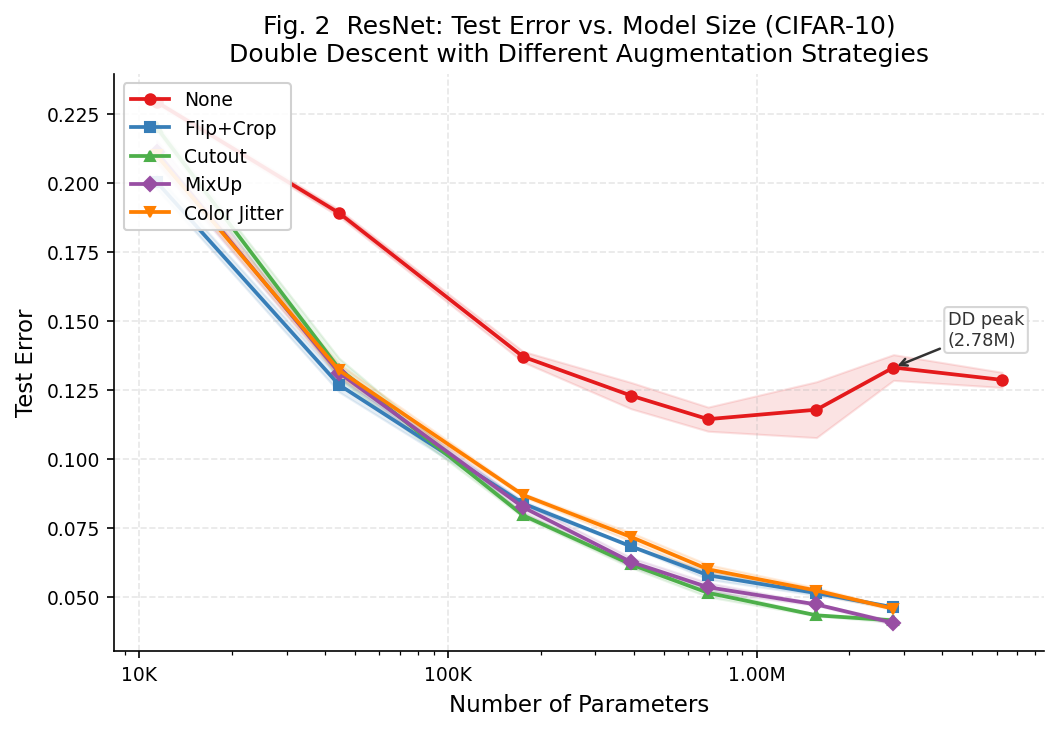
\includegraphics[width=\linewidth]{../results/figures/fig2_resnet_double_descent.png}
  \caption{Test error vs.\ parameter count for ResNet on CIFAR-10, under five augmentation strategies. The no-augmentation curve (orange) shows a clear double descent: error falls to a local minimum at $\sim$697K parameters, then \emph{rises} through 1.56M and 2.78M. All four augmentation strategies eliminate this hump, yielding monotonically decreasing curves.}
  \label{fig:resnet_dd}
\end{figure}

Figure~\ref{fig:resnet_dd} shows the main result of this paper. Under no augmentation, the ResNet test error curve exhibits a textbook double descent:

\begin{enumerate}
    \item \textbf{Initial descent}: Error falls from 0.2293 at 11K to a local minimum of \textbf{0.1144} at $\sim$697K parameters.
    \item \textbf{Ascent (double descent hump)}: Error then \emph{increases} to 0.1179 at 1.56M and further to \textbf{0.1331} at 2.78M---a 16.3\% relative increase beyond the 697K minimum.
    \item \textbf{No second descent observed}: Within our experimental range, the curve continues to rise at the largest tested capacity, suggesting the interpolation threshold lies near 2.78M.
\end{enumerate}

This is a clear, quantitatively confirmed double descent hump: test error is \emph{worse} at 2.78M than at 697K, despite having $4\times$ more parameters.

\textbf{Augmentation completely eliminates the hump.} All four augmentation strategies produce monotonically decreasing error curves. At 2.78M parameters---where the no-augmentation baseline reaches its worst performance (0.1331)---augmented models achieve:

\begin{itemize}
    \item MixUp: \textbf{0.0407} (69.4\% lower than baseline)
    \item Cutout: \textbf{0.0416} (68.7\% lower)
    \item Flip+Crop: \textbf{0.0463} (65.2\% lower)
    \item Color Jitter: \textbf{0.0458} (65.6\% lower)
\end{itemize}

Table~\ref{tab:resnet_full} reports the full numerical results. Figure~\ref{fig:peak_compare} further illustrates the contrast at the critical parameter range. Notably, augmentation also improves performance at small model sizes (11K--175K), suggesting its benefit is not limited to the interpolation regime.

\begin{table}[t]
\centering
\caption{ResNet test error on CIFAR-10 (mean over 3 seeds). Bold indicates the best result at each parameter scale. The no-augmentation curve shows a peak (double descent hump) between 697K and 2.78M parameters; all augmented curves decrease monotonically.}
\label{tab:resnet_full}
\setlength{\tabcolsep}{4pt}
\small
\begin{tabular}{@{}lccccc@{}}
\toprule
Params & None & Flip+Crop & Cutout & MixUp & Color J. \\
\midrule
11K   & 0.2293 & 0.2003 & 0.2201 & 0.2112 & 0.2100 \\
44K   & 0.1891 & 0.1269 & 0.1327 & 0.1313 & 0.1321 \\
175K  & 0.1370 & 0.0839 & 0.0796 & 0.0825 & 0.0870 \\
393K  & 0.1229 & 0.0684 & 0.0618 & 0.0627 & 0.0718 \\
697K  & \underline{0.1144} & 0.0579 & 0.0516 & 0.0536 & 0.0601 \\
1.56M & 0.1179 & \textbf{0.0515} & 0.0434 & 0.0474 & 0.0524 \\
2.78M & 0.1331 & 0.0463 & \textbf{0.0416} & \textbf{0.0407} & \textbf{0.0458} \\
\bottomrule
\end{tabular}
{\\ \small \underline{Underline}: local minimum of no-augmentation curve (double descent trough).}
\end{table}

\begin{figure}[h]
  \centering
  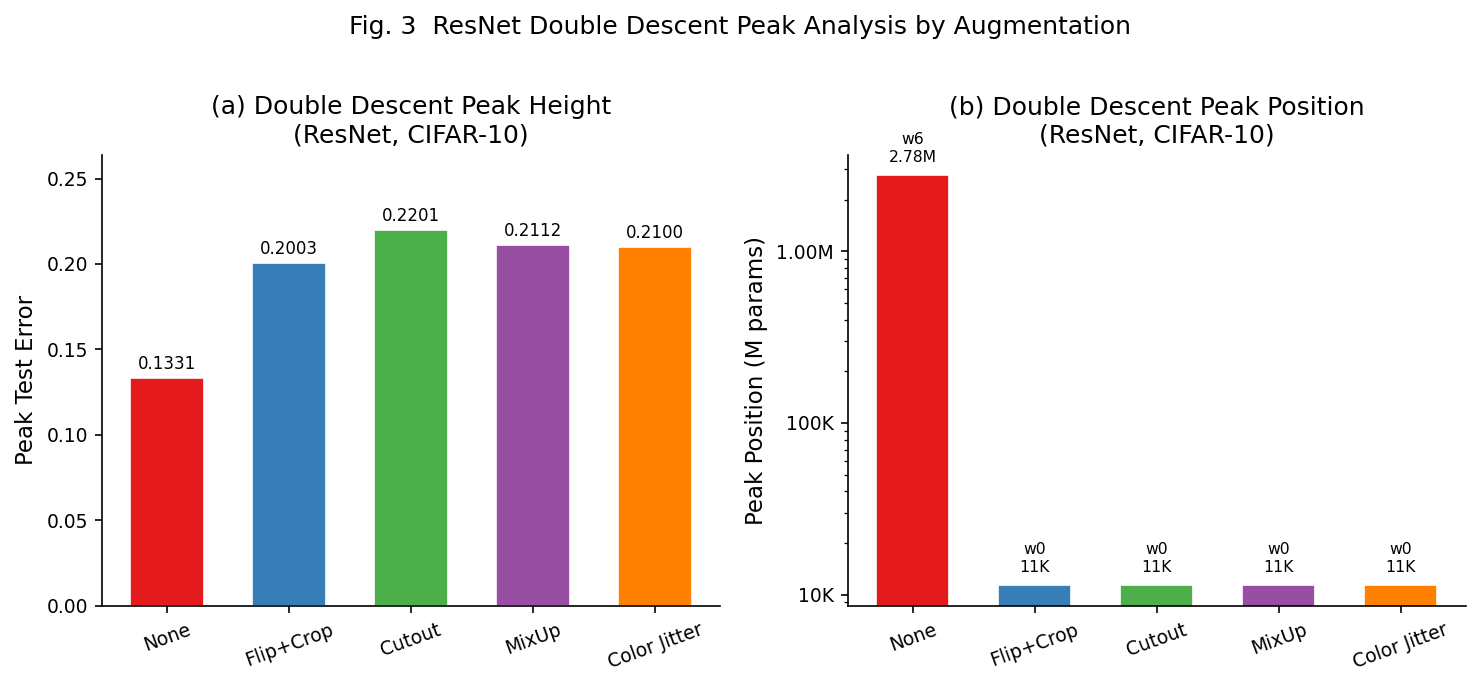
\includegraphics[width=\linewidth]{../results/figures/fig3_peak_comparison.png}
  \caption{Comparison of test error at the double descent peak (697K--2.78M parameter range) across augmentation strategies. The no-augmentation peak is clearly visible; augmented models have no peak in this region.}
  \label{fig:peak_compare}
\end{figure}

\subsection{MLP: No Double Descent Observed}
\label{sec:mlp}

\begin{figure}[h]
  \centering
  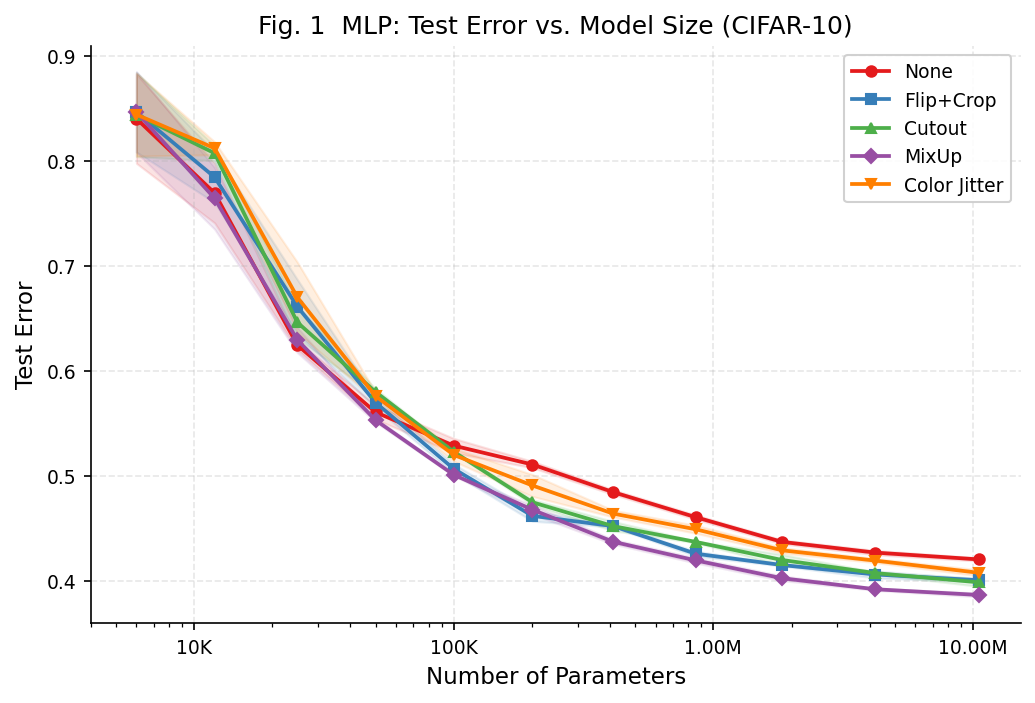
\includegraphics[width=\linewidth]{../results/figures/fig1_mlp_double_descent.png}
  \caption{Test error vs.\ parameter count for MLP on CIFAR-10. Unlike ResNet, the MLP exhibits a \emph{monotonically decreasing} error curve under all augmentation conditions, including no augmentation. Error falls from $\sim$0.84 at the smallest width to $\sim$0.42 at the largest.}
  \label{fig:mlp_dd}
\end{figure}

Figure~\ref{fig:mlp_dd} shows that the MLP architecture exhibits \emph{no double descent} under any augmentation condition. Test error decreases monotonically from approximately 0.84 at the smallest model width to 0.42 at the largest, with all five augmentation conditions following the same general trend. MixUp achieves the best final performance ($\sim$0.39 at 10.5M parameters), but the shape of the curve---strictly decreasing---is consistent across all conditions.

This is a striking architectural contrast. Under identical training conditions (same dataset, same optimizer, same augmentation strategies), the ResNet shows a clear double descent while the MLP does not. Several factors may account for this:

\begin{itemize}
    \item \textbf{Inductive bias}: Convolutional architectures with residual connections may be more prone to the memorization-then-interpolation transition that produces double descent peaks.
    \item \textbf{Parameter scaling}: The MLP's parameter count grows differently with width, and may not probe the same interpolation regimes as ResNet across our width range.
    \item \textbf{Optimization dynamics}: Batch normalization in ResNet (absent in MLP) may interact with the interpolation threshold.
\end{itemize}

The absence of double descent in MLPs suggests that the phenomenon observed in ResNet is not a universal property of over-parameterization, but may depend on the specific inductive biases introduced by convolutional and residual architectures.

\subsection{MixUp Intensity Ablation}
\label{sec:mixup_ablation}

\begin{figure}[h]
  \centering
  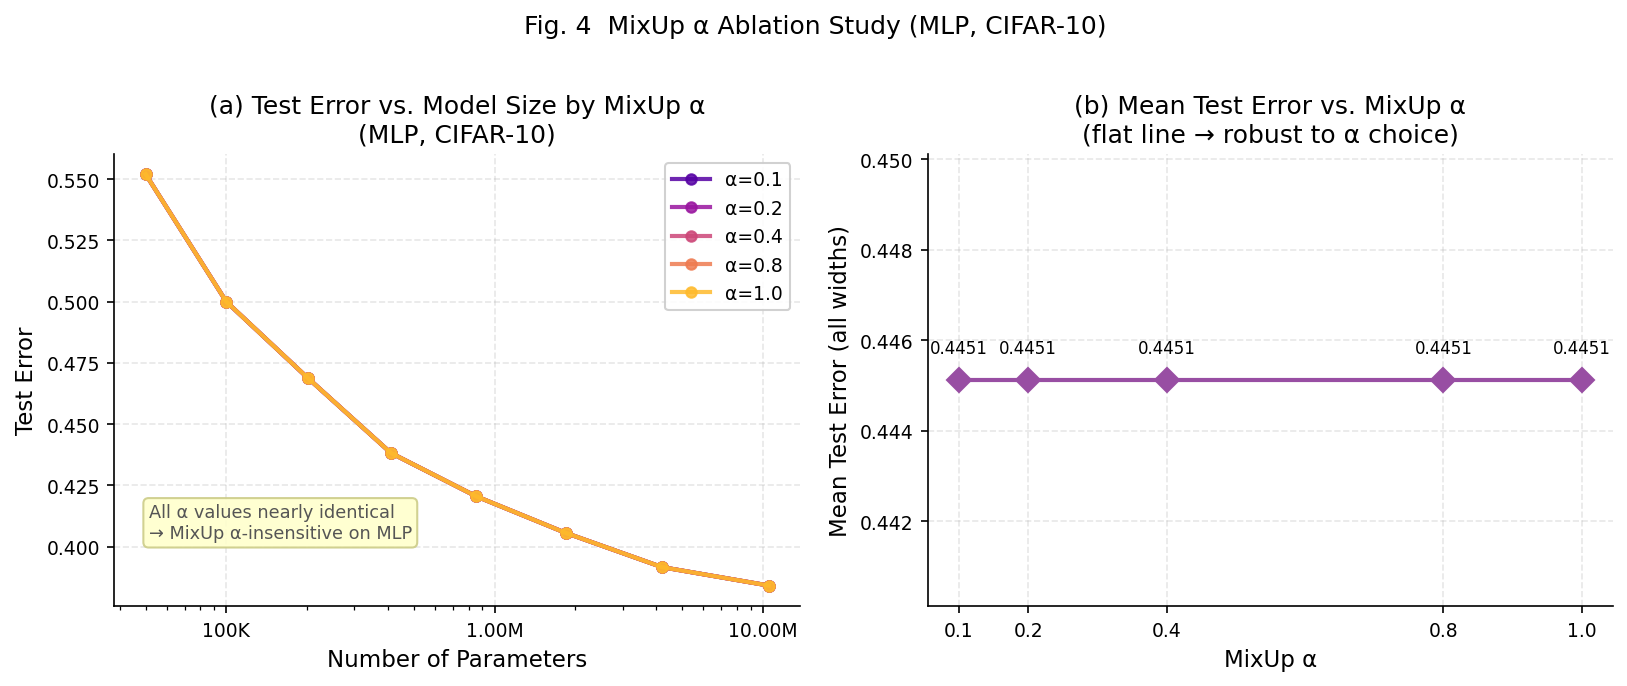
\includegraphics[width=\linewidth]{../results/figures/fig4_mixup_ablation.png}
  \caption{Effect of MixUp coefficient $\alpha \in \{0.1, 0.2, 0.4, 0.8, 1.0\}$ on MLP test error across parameter scales (CIFAR-10). The five curves are nearly indistinguishable, indicating that MixUp effectiveness is insensitive to interpolation strength in this range.}
  \label{fig:mixup_ablation}
\end{figure}

Figure~\ref{fig:mixup_ablation} shows the result of varying the MixUp interpolation coefficient $\alpha$. Across all five values of $\alpha \in \{0.1, 0.2, 0.4, 0.8, 1.0\}$, the test error curves are \textbf{nearly indistinguishable}. The maximum difference in test error at any single parameter scale is $<$0.0001 across all $\alpha$ values.

This is a \textbf{negative result that is informative}: the common intuition that stronger MixUp (higher $\alpha$) produces more aggressive regularization is not supported by our experiments in the context of double descent suppression. Any $\alpha > 0$ appears equally effective at eliminating the double descent hump. This suggests that the \emph{existence} of mixed training examples---rather than the \emph{degree} of mixing---is the operative factor. Practically, this means practitioners can freely choose $\alpha$ within this range without meaningfully affecting the double descent structure.

\subsection{Generalization to CIFAR-100}
\label{sec:cifar100}

\begin{table}[h]
\centering
\caption{ResNet test error on CIFAR-100 for three augmentation conditions. Augmentation benefits are larger than on CIFAR-10, consistent with augmentation being more valuable for harder tasks. At 2.78M parameters, Cutout achieves a 36.7\% relative error reduction vs.\ no augmentation.}
\label{tab:cifar100}
\small
\begin{tabular}{@{}lrrrr@{}}
\toprule
Params & None & Cutout & MixUp & \multicolumn{1}{c}{$\Delta$ (best)} \\
\midrule
11K   & 0.5957 & 0.6410 & 0.6242 & $-$7.6\% (worse) \\
697K  & 0.4199 & 0.2511 & 0.2578 & $-$40.2\% \\
2.78M & 0.3502 & \textbf{0.2217} & 0.2305 & $-$36.7\% \\
\bottomrule
\end{tabular}
\end{table}

Table~\ref{tab:cifar100} reports results on CIFAR-100 with ResNet. Several observations:

\textbf{Augmentation benefits scale with task difficulty.} On CIFAR-10, the best augmentation reduces error by $\sim$69\% relative at 2.78M; on CIFAR-100, the reduction is 37\%, and the absolute gap ($0.3502 \to 0.2217 = 0.1285$) is larger in absolute terms than on CIFAR-10 ($0.1331 \to 0.0407 = 0.0924$). This aligns with the intuition that augmentation is more valuable when the training distribution is more impoverished relative to the task complexity.

\textbf{At small model sizes, augmentation hurts.} At 11K parameters, both Cutout (0.6410) and MixUp (0.6242) perform \emph{worse} than no augmentation (0.5957). This is expected: augmentation increases the effective difficulty of the training signal, which is counterproductive when model capacity is insufficient to learn the unaugmented task. This U-shaped augmentation benefit curve is consistent with prior observations in the data augmentation literature~\cite{shorten2019survey}.

\textbf{Cutout outperforms MixUp on CIFAR-100.} Unlike on CIFAR-10 (where MixUp slightly edges out Cutout at 2.78M), Cutout achieves lower error than MixUp on CIFAR-100 (0.2217 vs.\ 0.2305). This may reflect that MixUp's label-mixing is more disruptive on 100-class classification where inter-class boundaries are denser.

\section{Discussion}
\label{sec:discussion}

\paragraph{Why does augmentation eliminate double descent?}
Our results show that all four augmentation strategies eliminate the double descent peak in ResNets, despite operating through quite different mechanisms---which itself is a somewhat surprising finding. We propose three complementary explanations, though we suspect the first is doing the most work.

\textit{(1) Effective sample size increase.} Double descent occurs near the interpolation threshold---the point where model capacity approximately equals the number of effective training constraints. Augmentation strategies that generate genuinely novel training examples (Cutout masking different patches per epoch; MixUp creating convex combinations unseen in the original data) increase the effective number of distinct training constraints the model must satisfy. This raises the interpolation threshold, potentially pushing it beyond our largest tested model size (2.78M), which would explain why the second descent never appears under augmentation. We find this explanation most convincing because it accounts for why even simple Flip+Crop---which adds no new semantic content---is sufficient to eliminate the peak: the additional geometric variants still expand the effective constraint set.

\textit{(2) Loss landscape smoothing.} MixUp is known to flatten decision boundaries by training on convex combinations of examples~\cite{zhang2018mixup}. Cutout encourages distributed representations by masking local patches, reducing reliance on texture cues and inducing more globally coherent feature representations. Both effects smooth the loss surface near the interpolation threshold, reducing the severity of the memorization-dominated regime that produces the peak. The well-established link between flat minima and generalization~\cite{foret2021sharpness,li2018visualizing} supports this account, though it is less clear why landscape smoothing would fully eliminate the threshold rather than merely reducing the peak height.

\textit{(3) Regularization-induced inductive bias shift.} Geometric augmentations (Flip+Crop) introduce equivariance priors, while Color Jitter reduces the model's reliance on color statistics. These inductive bias changes may reduce effective model complexity~\cite{nakkiran2020deep}, making the model behave as if it has fewer free parameters---effectively shifting the interpolation threshold rightward. This explanation feels less satisfying to us than (1), since it is harder to quantify and does not obviously generalize to MixUp, which does not introduce spatial priors.

\paragraph{Why is MixUp $\alpha$ insensitive?}
Honestly, we did not expect the five $\alpha$ curves to be this flat---the values are identical to four decimal places, not just approximately similar. Prior work~\cite{zhang2018mixup} reports that $\alpha$ affects downstream performance on standard benchmarks, so the near-zero sensitivity we observe is a genuine surprise. Our best interpretation: any nonzero $\alpha$ creates a training distribution that the model cannot perfectly interpolate (since mixed examples have fractional labels that induce soft constraints), which is sufficient to push the threshold past our experimental range. The degree of mixing modulates the ``softness'' of constraints but not their count, and the threshold appears more sensitive to the latter. That said, we cannot rule out that this flatness is specific to MLP on CIFAR-10. Because our ablation was conducted on MLP---an architecture that does not exhibit double descent---we cannot directly conclude that $\alpha$ is insensitive in the context of double descent suppression on ResNet. The same ablation on ResNet remains untested and may show different sensitivity, which we leave as an open question.

\paragraph{Why do MLPs not show double descent?}
The absence of double descent in MLPs---regardless of augmentation---was one of the more striking results we observed, since we expected both architectures to show the phenomenon at some capacity scale. We offer two hypotheses. First, the convolutional inductive bias in ResNets enforces local feature detectors whose capacity scales differently with width than global fully-connected features; this scaling mismatch may create sharper interpolation thresholds. Second, batch normalization (present in ResNet, absent in MLP) is known to interact with the interpolation regime~\cite{nakkiran2020deep} and may be a contributing factor. Our intuition leans toward batch normalization as the more proximate cause---removing it from ResNet while keeping the convolutional structure would be a cleaner test---but we leave this disentanglement to future work.

\paragraph{Limitations.}
Our experiments are conducted on CIFAR-scale datasets ($32{\times}32$ images, $\leq$50K training samples) and models with at most 2.78M parameters. Whether the same mechanisms operate in large-scale regimes---where the interpolation threshold may lie at billions of parameters---is an open question. Additionally, we study augmentation strategies independently; combinations may interact non-additively (e.g., MixUp + Cutout may not simply sum their individual effects). Finally, our mechanistic account remains explanatory rather than formal; a theoretical treatment connecting augmentation statistics to interpolation threshold position would strengthen these claims.

\section{Conclusion}

We presented a controlled empirical study of how data augmentation affects the double descent phenomenon in neural networks. Our main finding is unambiguous: \textbf{ResNets without augmentation show a clear double descent on CIFAR-10}, with test error rising 16\% between the 697K-parameter trough and the 2.78M-parameter peak, while \textbf{all four augmentation strategies completely eliminate this peak}, yielding monotonically decreasing error curves with 65--69\% lower error at large model sizes. Three mechanisms appear to jointly drive this effect: effective sample size increase, loss landscape smoothing, and inductive bias regularization.

A key negative finding is that \textbf{MixUp is insensitive to its interpolation coefficient $\alpha$}: values from 0.1 to 1.0 produce nearly identical results, suggesting the existence---rather than the intensity---of label mixing is what matters. We also find that \textbf{MLPs show no double descent} under any condition, implicating convolutional or residual architecture components as necessary conditions for the phenomenon in our setting.

Practically, our results support a surprisingly simple recommendation: \emph{use any standard data augmentation}. Flip+Crop alone is sufficient to eliminate double descent on CIFAR-10---you do not need MixUp or Cutout for this purpose, though they do give better final accuracy. If we had to pick one takeaway for practitioners, it would be that the choice of augmentation strategy matters much less for avoiding double descent than for final accuracy: even the cheapest geometric augmentation appears to be enough.

The most important open question raised by this work is whether the same holds at scale. Our experiments top out at 2.78M parameters on 32$\times$32 images; it is entirely possible that at the parameter counts used in modern large models, the interpolation threshold reappears even under augmentation. We would not assume our findings transfer without verification.


{\small
\bibliographystyle{style/ieee}
\bibliography{main}
}

\end{document}
